\section{The shattering depth}
\label{sec:depth}

The third round of computation for this chapter asked a question that the earlier rounds had not: when the bottom level set $\{ S \le 1 \}$ of a board shatters, does the next level set $\{ S \le 2 \}$ shatter too? The answer, on every unconditioned board we have examined, is no, and it changes what the program should ask for.

\begin{problem}[Swap connectivity of the second level set]
Determine the least $m_c(N)$ such that $\{ S \le m_c \}$ is connected under swaps for the unconditioned $N$ queens problem.
\end{problem}

Status. Resolved for $N \le 11$ by exhaustive enumeration of all $N!$ placements with a breadth first search over swaps at every energy threshold. Table~\ref{tab:levelsets} gives the number of swap components of $\{ S \le m \}$ for $m = 0, 1, 2$. The level set $\{ S \le 2 \}$ is connected for every $N$ from $4$ to $11$, so $m_c(N) \le 2$ in this range, and $m_c(N) = 2$ except at $N = 8$, where $\{ S \le 1 \}$ is already connected. At $m = 1$ the level set has many components for $N \ge 9$ ($69$, $253$ and $1121$ for $N = 9$, $10$, $11$), almost all of them small clusters of near solutions containing no solution, as the earlier table showed; at $m = 2$ every one of them is absorbed into a single component. We conjecture that $m_c(N) = 2$ for all $N \ge 9$. The conjecture is needed in the sketch of the conditional FPRAS for $Q(N)$ in Chapter~\ref{ch:program}, where it replaces an argument from monotonicity that the first draft of that proof wrongly relied on: the level sets are nested but the connectivity of a larger one does not follow from the connectivity of a smaller one, and the computation is what supports the claim.

\begin{table}[t]
\centering
\small
\caption{Swap components of the level sets $\{ S \le m \}$ of the unconditioned problem, by exhaustive enumeration. For each $N$: the size of $\{ S \le m \}$ and the number of swap components, for $m = 0$, $1$ and $2$. The level set $\{ S \le 2 \}$ is connected for every $N$ shown.}
\label{tab:levelsets}
\begin{tabular}{rrrrrrr}
\toprule
$N$ & $|\{S \le 0\}|$ & comps & $|\{S \le 1\}|$ & comps & $|\{S \le 2\}|$ & comps \\
\midrule
4 & 2 & 2 & 10 & 2 & 16 & 1 \\
5 & 10 & 10 & 10 & 10 & 66 & 1 \\
6 & 4 & 4 & 64 & 10 & 224 & 1 \\
7 & 40 & 36 & 192 & 22 & 872 & 1 \\
8 & 92 & 84 & 980 & 1 & 3844 & 1 \\
9 & 352 & 304 & 3728 & 69 & 20376 & 1 \\
10 & 724 & 612 & 15128 & 253 & 106056 & 1 \\
11 & 2680 & 2128 & 70336 & 1121 & 584024 & 1 \\
\bottomrule
\end{tabular}
\end{table}

A proof of $m_c(N) \le 2$ would be the natural base of a canonical path\index{canonical paths} argument on $\{ S \le 2 \}$. We do not have one. A proof that $m_c(N) \le c$ for some constant $c$ would already have consequences, since the ratio $N(0) / |\{ S \le c \}|$ should then be at least inverse polynomial, of order $N^{-c}$ by the heuristic that each additional attack can be placed in about $N$ ways; a bound $m_c(N) \le cN$ would not, since by the rate function of Chapter~\ref{ch:entropy} the ratio $N(0) / |\{ S \le cN \}|$ is then exponentially small. The paragraph below explains why the distinction matters.

\begin{problem}[The shattering depth of a board]
For a board $B$ with completions, define the solution depth $m_s(B)$ as the least $m$ such that all completions of $B$ lie in one swap component of the conditioned level set $\{ S \le m \}$, and the shattering depth $m_c(B)$ as the least $m$ such that $\{ S \le m \}$ is itself connected. Determine the distributions of $m_s(B)$ and $m_c(B)$ over random boards and their growth over hard boards.
\end{problem}

Status. The random queens completion model of the previous section showed that random conditioning fragments $\{ S \le 1 \}$. We have now run that model on $300$ instances per $k$ at $N = 12$ and $150$ at $N = 13$, with the fixed queens chosen uniformly subject to pairwise non attack and the instance kept if it has a completion, and the results are in Table~\ref{tab:random2}. About half of the random boards with two to four fixed queens have their completions in more than one component of $\{ S \le 1 \}$: $47\%$ at $N = 12$ with $k = 2$, $62\%$ with $k = 3$, and $54\%$ to $57\%$ at $N = 13$ with $k = 3$ and $4$. The worst boards are severely shattered. A board at $N = 12$ with two fixed queens, at row $0$ column $2$ and row $11$ column $0$, has $42$ completions spread over $30$ components of $\{ S \le 1 \}$, the largest holding $5$ (this board comes from a separate random draw of boards at the same size, not from the $300$ instances of the table, whose most shattered board at $N = 12$ with $k = 2$ has $22$ components); a board at $N = 13$ with three fixed queens has $17$ completions in $15$ components. A greedy adversarial search that moves one fixed queen at a time to increase the number of solution components finds, at $N = 12$ with three fixed queens, a board with $16$ completions in $12$ components and one with $39$ completions in $13$, and with four fixed queens a board whose six completions are all isolated from one another. Shattering of the bottom level set is therefore not rare under random conditioning and can be made severe by a weak adversary, at sizes where the solution derived conditioning of Table~\ref{tab:conditioned} shows nothing of the kind. This is the planted versus random distinction of the satisfiability literature appearing in the queens: a board that was cut out of a solution keeps that solution's component intact, and a board that was not has no such guarantee.

\begin{table}[t]
\centering
\small
\caption{Random boards with $k$ fixed queens and at least one completion, $300$ instances per row at $N = 12$ and $150$ at $N = 13$: mean number of completions, fraction of instances whose completions lie in more than one component of $\{ S \le 1 \}$, mean and maximum number of solution components, and mean and minimum fraction of completions in the largest component.}
\label{tab:random2}
\footnotesize
\begin{tabular}{rrrrrrrr}
\toprule
$N$ & $k$ & mean $N(0)$ & multi & comps & max & giant & min \\
\midrule
12 & 2 & 121.8 & 0.47 & 2.50 & 22 & 0.977 & 0.161 \\
12 & 3 & 15.6 & 0.62 & 2.52 & 11 & 0.826 & 0.111 \\
12 & 4 & 3.2 & 0.46 & 1.63 & 5 & 0.799 & 0.200 \\
12 & 5 & 1.5 & 0.18 & 1.21 & 4 & 0.914 & 0.250 \\
13 & 3 & 59.6 & 0.54 & 2.59 & 15 & 0.944 & 0.118 \\
13 & 4 & 8.7 & 0.57 & 2.22 & 10 & 0.766 & 0.143 \\
13 & 5 & 2.5 & 0.40 & 1.57 & 4 & 0.810 & 0.250 \\
\bottomrule
\end{tabular}
\end{table}

The new fact is what happens one and two levels up. For each of the worst boards we enumerated the conditioned level sets $\{ S \le m \}$ for $m = 2, 3, 4$ and found their swap components. On every one of them all completions lie in a single component of $\{ S \le 2 \}$. The board with $42$ completions in $30$ components of $\{ S \le 1 \}$ has them in one component of $\{ S \le 2 \}$; so does the adversarial board with $39$ completions in $13$ components, and the board with six isolated completions. In every case examined the solution depth is $m_s(B) = 2$: the near solutions with one attack are too sparse to bridge the completions, and the placements with two attacks are dense enough. The level set $\{ S \le 2 \}$ is not itself connected on these boards: it has $94$, $5$ and $13$ components, all but one of them islands of two attack placements that contain no completion. These islands matter, because a chain that samples $\{ S \le 2 \}$ from a completion never reaches them and the fraction of ground states it reports is biased by their mass. One level higher they are absorbed: $\{ S \le 3 \}$ is connected on the first two boards and $\{ S \le 4 \}$ on the third, so the shattering depth is $m_c(B) = 3$ or $4$. On forty random boards with two fixed queens and forty with three, $m_s(B)$ is $1$ on fifteen and $2$ on twenty five of each forty, never more, and $m_c(B)$ is $3$ on seventy five of the eighty, $2$ on three, and $4$ on two. Table~\ref{tab:depth} gives the counts for the three boards, and with them the price of climbing: the ratio $N(0) / |\{ S \le m_c \}|$ is between $0.0005$ and $0.002$ on these boards and about $0.001$ on average over the random ones, against a ratio $N(0) / |\{ S \le 1 \}|$ near $0.04$ on unconditioned boards ($0.039$ at $N = 12$). The price of two levels is a factor of thirty to forty in the bottom ratio, and so of thirty to forty in the number of samples a Bernoulli estimate of that ratio needs.

\begin{table}[t]
\centering
\small
\caption{Depths of three severely shattered boards at $N = 12$. The fixed queens are given as (row, column) pairs; $N(0)$ is the number of completions; for each $m$ the size of the conditioned level set $\{ S \le m \}$, its number of swap components, and the number of those containing a completion. The shattering depth is the first $m$ with one component: $3$, $3$ and $4$. The ratios $N(0) / |\{ S \le m_c \}|$ are $0.0005$, $0.0020$ and $0.0011$.}
\label{tab:depth}
\footnotesize
\begin{tabular}{p{3.2cm}rrrrr}
\toprule
board & $N(0)$ & $m$ & size & comps & with sol \\
\midrule
$(0,2)$, $(11,0)$ & 42 & 1 & 1285 & 447 & 30 \\
 & & 2 & 15549 & 94 & 1 \\
 & & 3 & 87763 & 1 & 1 \\
\midrule
$(7,11)$, $(10,5)$, $(11,10)$ & 39 & 1 & 515 & 98 & 13 \\
 & & 2 & 4335 & 5 & 1 \\
 & & 3 & 19126 & 1 & 1 \\
\midrule
$(0,7)$, $(1,11)$, $(8,10)$, $(11,8)$ & 6 & 1 & 49 & 23 & 6 \\
 & & 2 & 448 & 13 & 1 \\
 & & 3 & 1928 & 2 & 1 \\
 & & 4 & 5265 & 1 & 1 \\
\bottomrule
\end{tabular}
\end{table}

This changes the shape of the mixing conjecture. The vertical walk does not need the bottom rung; it needs some rung whose level set is connected and well mixed and whose ratio to the ground state is not too small. The following statement makes that precise.

\begin{theorem}[Rung skipping]
\label{thm:rungskip}
Let $B$ be a board with completions and let $m \ge m_c(B)$. Suppose the swap chain on the conditioned level set $\{ S \le j \}$ is irreducible and mixes in time $T$, polynomial in $N$, for every $j \ge m$, that $|\{ S \le j \}| / |\{ S \le j + 1 \}| \ge 1 / q(N)$ for every $j \ge m$ and a polynomial $q$, and that $N(0) / |\{ S \le m \}| \ge 1 / p(N)$ for a polynomial $p$. Let $K$ be the number of rungs above $m$, that is, the number of $j \ge m$ with $\{ S \le j \}$ not the whole board. Then the vertical walk that estimates $N(0) / |\{ S \le m \}|$ directly, as the fraction of ground states among samples from $\{ S \le m \}$, and the ratios $|\{ S \le j \}| / |\{ S \le j + 1 \}|$ for $j \ge m$ by the product estimator, is an FPRAS for the completion count with cost $O((K^3 q(N) + p(N)) \epsilon^{-2} T \log (K/\delta))$ for confidence $1 - \delta$.
\end{theorem}

\begin{proof}
The bottom ratio is a Bernoulli mean with success probability at least $1/p(N)$, so $O(p(N) \epsilon^{-2} \log (1/\delta))$ samples give relative error $\epsilon / 2$ with the stated confidence. Each rung ratio $|\{ S \le j \}| / |\{ S \le j + 1 \}|$ above $m$ is a Bernoulli mean, under the uniform law on $\{ S \le j + 1 \}$, of at least $1/q(N)$, by the rung ratio hypothesis, so $O(q(N) K^2 \epsilon^{-2} \log (K/\delta))$ samples from a chain with mixing time $T$ estimate it to relative error $\epsilon / (2K)$, and the product of the $K$ estimates has relative error about $\epsilon / 2$, so that with the bottom ratio the total is within a constant multiple of $\epsilon$, which rescaling $\epsilon$ removes; this is the argument of the conditional FPRAS theorem of Chapter~\ref{ch:program}, run on the conditioned level sets instead of the unconditioned ones. The condition $m \ge m_c(B)$ is necessary rather than sufficient for the mixing hypothesis: below the shattering depth the level set is disconnected and no chain on it is irreducible, and above it irreducibility at every level $j \ge m$ is part of what is assumed, since the connectivity of $\{ S \le m \}$ does not by itself imply that of $\{ S \le m + 1 \}$. Solution depth is not enough: a chain on $\{ S \le m_s \}$ started from a completion samples the completion component uniformly but never the islands, and the ground state fraction it reports is too large by the factor of the island mass.
\end{proof}

The theorem relocates the question. On the boards examined at $N = 12$, $m = 3$ suffices on all but two of eighty, $m = 4$ on those two, and larger $N$ need $m = 4$ more often (Table~\ref{tab:depthgrowth}), and the price is a factor of thirty to forty in the bottom ratio, which is nothing. The mixing conjecture for hard boards is then not that $\{ S \le 1 \}$ shatters, which it demonstrably does on easy random boards as well, but that the shattering depth grows: that on reduction boards from hard formulas $m_c(B)$ is of order $N$ or larger, so that the first connected level set has exponentially more placements than completions and the Bernoulli estimate of the bottom ratio takes exponential time. Equivalently, the hardness lives not in the disconnection of one level set but in the depth to which the disconnection persists. We state this as the revised conjecture.

\begin{conjecture}[Shattering depth on hard boards]
\label{conj:shatterdepth}
There is a family of boards $B_N$ from the Gent Jefferson Nightingale reduction applied to hard formulas with $m_c(B_N) \ge c N$ for a constant $c > 0$, and for such boards the ratio $N(0) / |\{ S \le m_c(B_N) \}|$ is exponentially small in $N$.
\end{conjecture}

The conjecture is testable: the enumeration that found $m_c = 3$ on the random boards runs in seconds at $N = 12$, and on a reduction board of moderate size it would find the depth directly. Its negation at every size, $m_c(B) \le c$ for a constant $c$ on all boards, together with polynomial mixing above the depth, an inverse polynomial bound on $N(0) / |\{ S \le c \}|$ and on the rung ratios, would give $\NP = \RP$ by the rung skipping theorem and the main equivalence, and this is now the sharpest form of the program's Monte Carlo half that we can state: find the shattering depth of hard boards.

\begin{problem}[Queenon tilted proposals]
Does a swap proposal tilted towards the queenon density mix faster than the uniform swap on the bottom level set?
\end{problem}

Status. Resolved negatively at the sizes tested. Simkin\index{Simkin's theorem}'s queenon\index{queenon} is the limiting density of queen positions in a uniform solution, and one might hope that proposing swaps that move queens towards the dense parts of the board would raise the acceptance rate of the bottom rung chain. We estimated the density from the $73712$ solutions at $N = 13$, interpolated it to an $N \times N$ board, and ran the swap chain on $\{ S \le 1 \}$ with the pair $(i, j)$ proposed with probability proportional to $q(i, x_j) \, q(j, x_i)$, the product of the densities at the two squares the swap would occupy, with the Metropolis Hastings correction that keeps the uniform target. Figure~\ref{fig:queenon} shows the density and the comparison. The density is far from flat: along the middle row it is $1.42$ times uniform at the edges and $0.79$ at the centre, and along the top row $0.49$ at the corners and $1.42$ at the centre, the pattern that Simkin's queenon predicts. The tilt does not help. At $N = 12, 16, 20, 24$ the integrated autocorrelation times of the first row column are $246, 402, 775, 716$ proposals for the uniform swap and $312, 489, 956, 761$ for the tilted swap, with standard deviations over five runs of sixteen to forty eight percent, and the acceptance rates fall from $0.061, 0.046, 0.036, 0.032$ to $0.052, 0.040, 0.033, 0.029$. The tilted chain is slightly slower at every size. The reason is that the queenon is a one point marginal and the constraints are pairwise: the squares that are dense are dense because many solutions use them, not because a given near solution can be repaired by moving a queen there, and proposing moves towards them lowers the acceptance rate without shortening the repair paths. A proposal that could help would have to use the conditional density of a square given the other queens, which is the thing the chain is trying to sample. The problem that remains open is whether a two point tilt, using Simkin's bound on the density of attacking pairs, does any better; we expect not.

\begin{figure}[t]
\centering
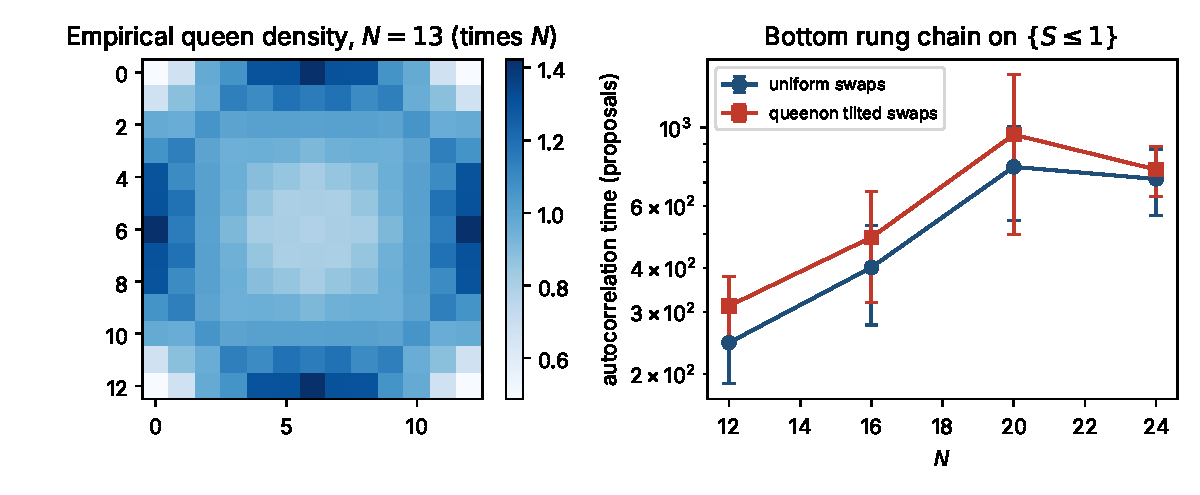
\includegraphics[width=\textwidth]{fig_queenon.pdf}
\caption{Left: the empirical queen density at $N = 13$, from all $73712$ solutions, scaled so that uniform is one. Right: autocorrelation time of the bottom rung chain with uniform and queenon tilted swap proposals, mean and standard deviation over five runs.}
\label{fig:queenon}
\end{figure}

